\chapter{Результати моделювання. Оцінка характеристик двигуна}\label{sec:model_results}

\section{Результати моделювання термодинамічних процесів у камері РРД}




За допомогою програмного комплексу відкритого доступу \texttt{Астра.4/рс} після верифікації моделі було проведено термодинамічний розрахунок дво- і трикомпонентних реакцій у камері трьох різних РРД, розглянутих у розділі~\ref{sec:model_conditions} за присутності компонентів паливної суміші та визначеної масової частки присадки (рис.~\ref{fig:RD-0120_add},~\ref{fig:11D123_add},~\ref{fig:SV-3_add}). Спад тяги після введення третього компонента розрахований на основі отриманих основних параметрів камери згоряння та сопла: тиску в ядрі потоку, питомого імпульсу, витратного і тягового комплексів та площі критики.

\begin{figure}
	\centering
	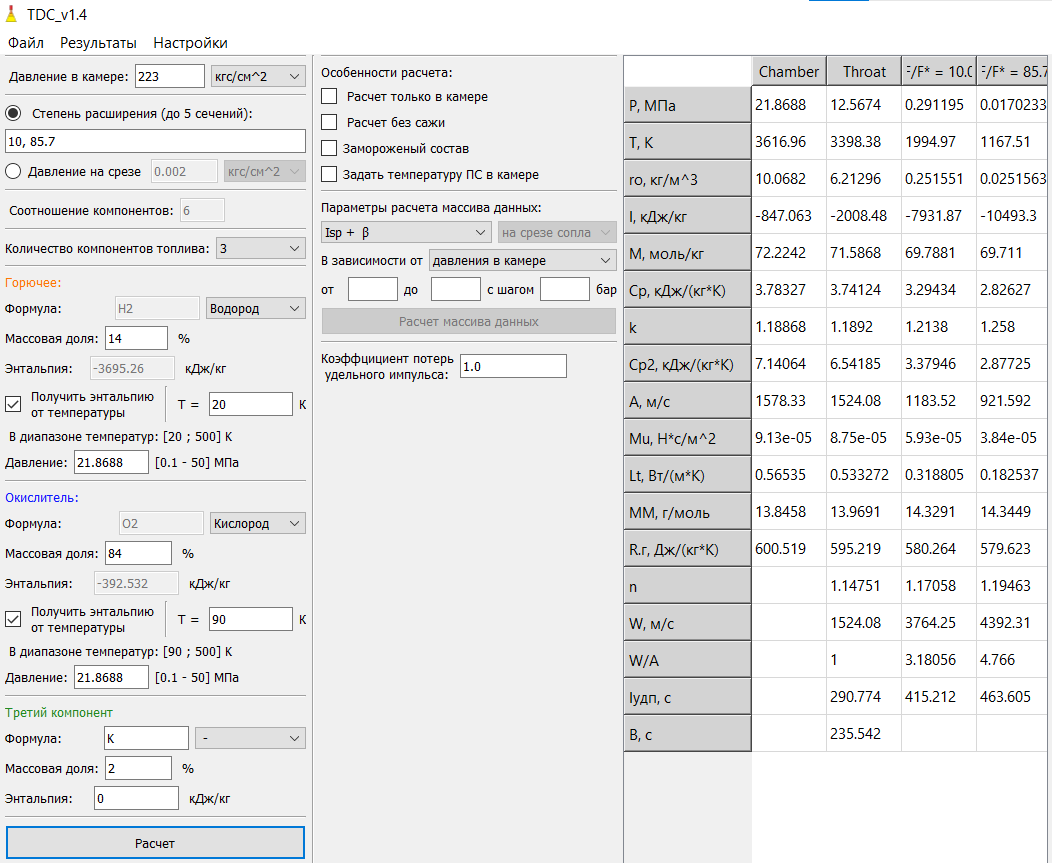
\includegraphics[width=0.5\textheight, angle=0,origin=c]{chapter_3/RD-0120_add.png}
	\caption{Розрахунок термо- і газодинамічних параметрів камери і визначених перерізів сопла двигуна РД-0120 за присутності частинок присадки (інтерфейс оболонки програмного комплексу \texttt{Астра.4/рс})}
	\label{fig:RD-0120_add}
\end{figure}

\begin{figure}
	\centering
	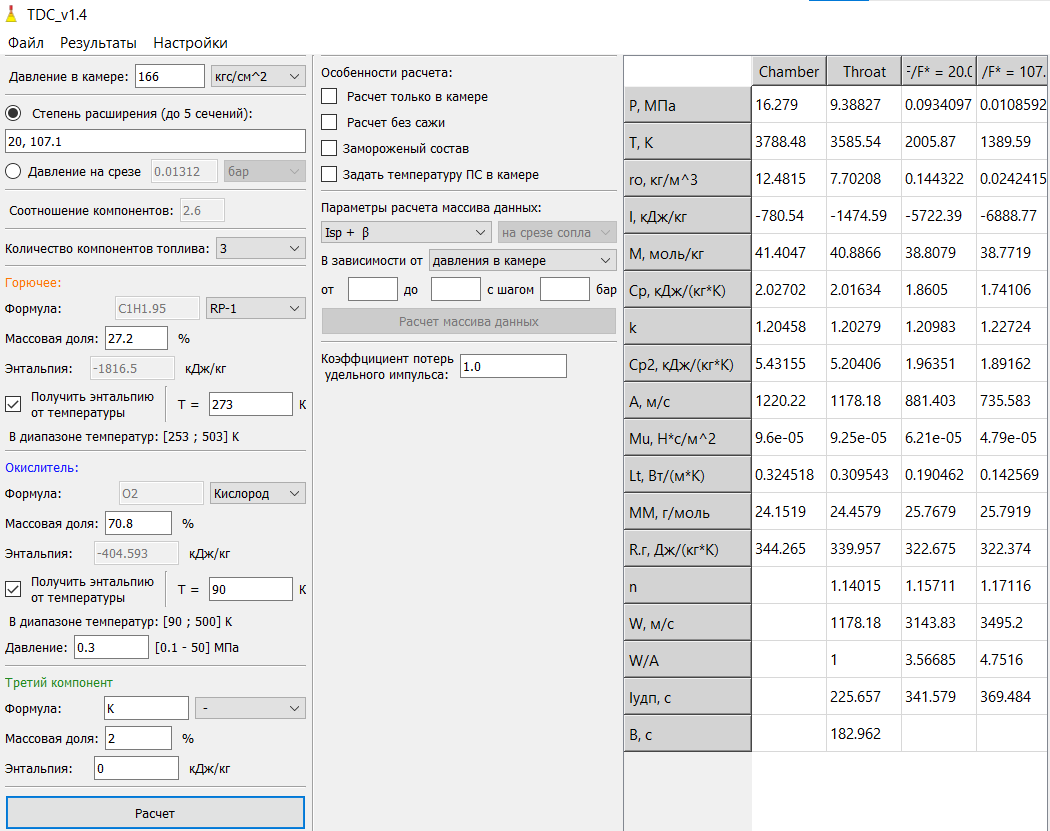
\includegraphics[width=0.5\textheight, angle=0,origin=c]{chapter_3/11D123_add.png}
	\caption{Розрахунок термо- і газодинамічних параметрів камери і визначених перерізів сопла двигуна 11Д123 за присутності частинок присадки (інтерфейс оболонки програмного комплексу \texttt{Астра.4/рс})}
	\label{fig:11D123_add}
\end{figure}

\begin{figure}
	\centering
	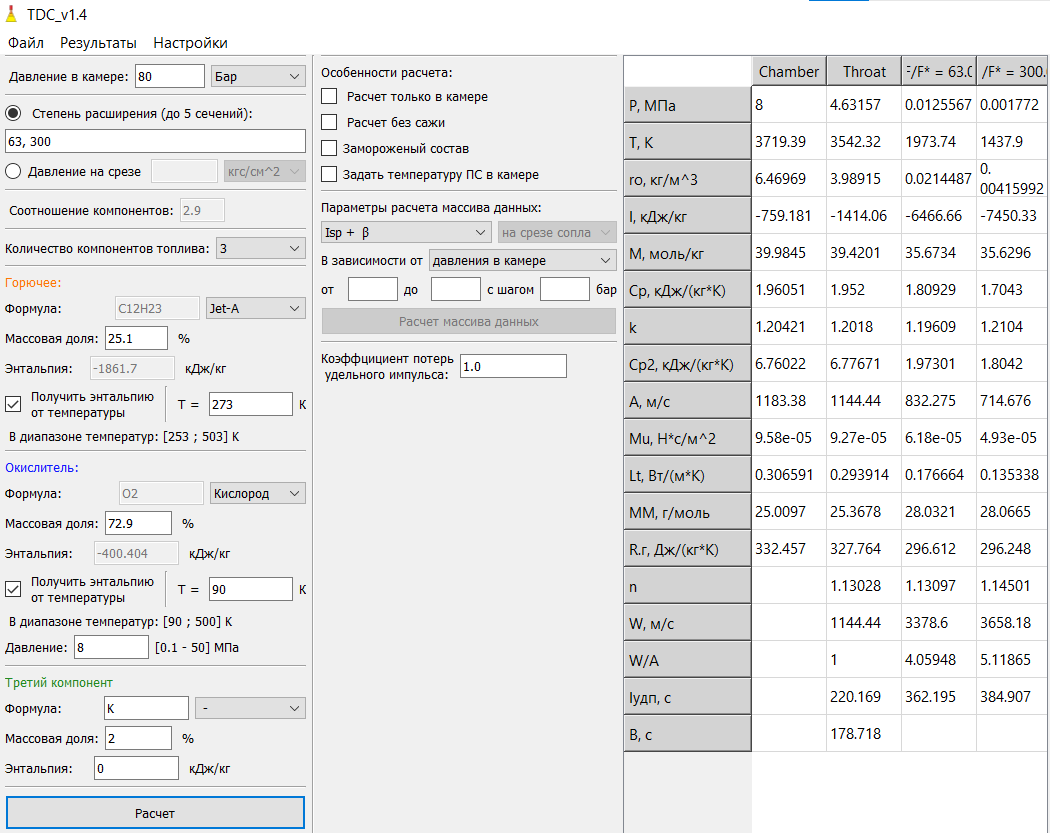
\includegraphics[width=0.5\textheight, angle=0,origin=c]{chapter_3/SV-3_add.png}
	\caption{Розрахунок термо- і газодинамічних параметрів камери і визначених перерізів сопла двигуна SV-3 за присутності частинок присадки (інтерфейс оболонки програмного комплексу \texttt{Астра.4/рс})}
	\label{fig:SV-3_add}
\end{figure}



Результати розрахунку для усіх трьох двигунів наведені у табл.~\ref{tab_LPRE}.

\begin{table}[h!]\centering\small
	\caption{Характеристики РРД за ТД-розрахунком у пакеті \texttt{Астра.4/рс}}
	\begin{tabular}{|l|c|c|c|c|c|c|}
		\hline
		\thead{} & \thead{РД-0120} & \thead{РД-120 (11Д123)} & \thead{Flight Control SV3}\\
		\hline
		Паливо 					& LH2+LOX & РГ-1+LOX & Jet A-1+LOX \\
		\hline
		Маса, кг 				& 3450    & 1125     & 140 \\
		\hline
		Тягооснащеність 		& 57,97   & 75,56    & 21,43 \\
		\hline
		Тяга, тс 				& 200	  & 85       & 3 \\
		\hline
		Питомий імпульс, м/с 	& 4462    & 3432     & 3482,55 \\
		\hline
		Спад тяги з присадкою (\%) & 1,018   & 0,991    & 0,942 \\
		\hline
	\end{tabular}
	\label{tab_LPRE}
\end{table}

%Застосована стандартна ініціалізація розрахунку, задана кількість ітерацій $1000$. Кратність ітерацій DPM - $2$. Верифікаційний розрахунок без введення присадки дійшов збіжності за 429 ітерацій.

%Отримані поля динамічного та повного тиску, температури, швидкості й числа Маха наведені на рис.~\ref{fig:pure_dyn_pressure},~\ref{fig:pure_tot_pressure},~\ref{fig:pure_temperature},~\ref{fig:pure_velocity_magn},~\ref{fig:pure_mach_number}. Помітний перший стрибок ущільнення за зрізом сопла, також наявна вторинна границя потоку. У камері спостерігається вигоряння водню у перших 3-4 см її довжини; далі переважну більшість маси робочого тіла становить вода, проте у перерізі камери тиск і температура досягають значень $8$ МПа і  $3850-3930$ К, близьких до заявлених авторами~\cite{VinciDataDLR} значень для двигуна на режимі, отже задана конфігурація відтворює термо- й газодинамічні параметри РРД.

%Перевірене значення тиску на зрізі сопла свідчить про спад тяги через різницю тисків (англ. pressure thrust) на $29.566$ кН, отже присутнє недорозширення сопла, властиве для двигунів верхніх ступеней та низького тиску навколишнього середовища.

%Проведені розрахунки потоків РРД з введенням частинок калію фракціями 5, 10, 20, 50 і 75 мкм; в результаті отримані траекторії частинок у реактивному струмені РРД, наведені на рис.~\ref{subfig1}~-~\ref{subfig5}. Варто помітити, що зі зменшенням розміру частинок вони рівномірніше розподіляються у перерізі потоку, що може свідчити про наближення до термодинамічної рівноваги між частинками присадки й потоком газу. Наведені траєкторії частинок з профілями швидкості, а також аналогічні траекторії з профілями температури показують, що потоки з присадкою фракцією 5 - 20 мкм мають розподіл значень, близький до розподілу у навколишньому реактивному струмені РРД. Граничні верхні значення у розподілі температур відхиляються у межах 1\%, швидкостей - 0.2, 12.9 і 8.9\% відповідно. У фракції 50 мкм ці відхилення становлять 27\% ($v$) і ті ж 5\% ($T$), для 75 мкм маємо 32.7\% ($v$), 9.2\% ($T$).


\section{Взаємна інтеграція установок і її вплив на результуючі параметри}

\begin{figure}
	\centering
	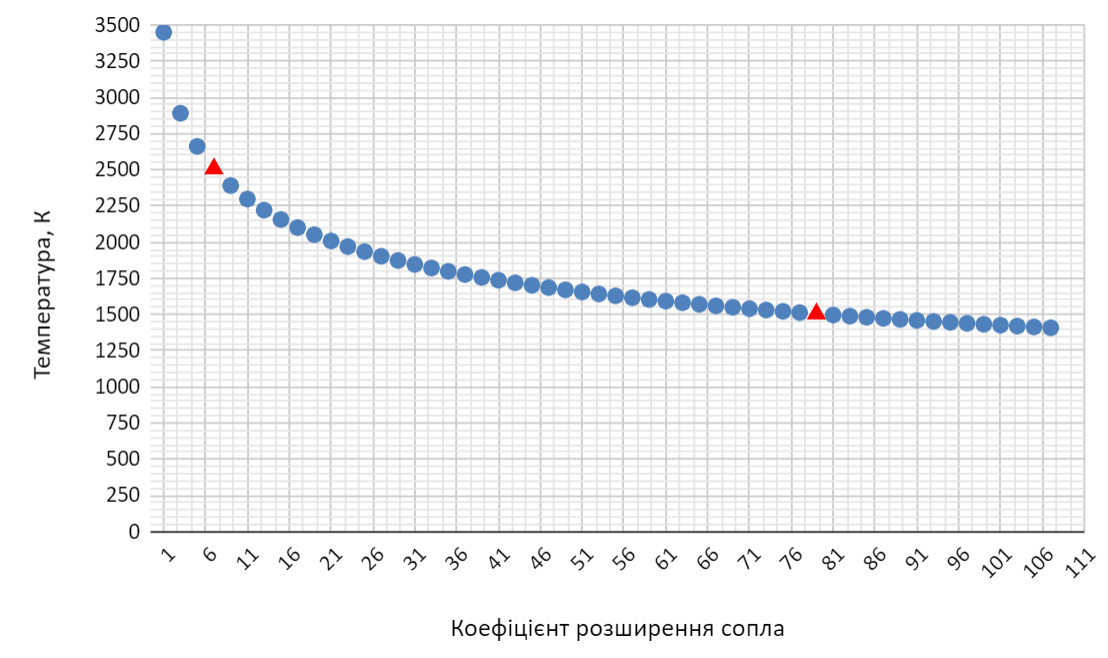
\includegraphics[width=0.7\textheight, angle=0,origin=c]{chapter_3/11D123_T(epsilon).png}
	\caption{Профіль температури у соплі 11Д123; червоним показані перерізи розташування МПД-каналу}
	\label{fig:11D123_T(epsilon)}
\end{figure}

\begin{figure}
	\centering
	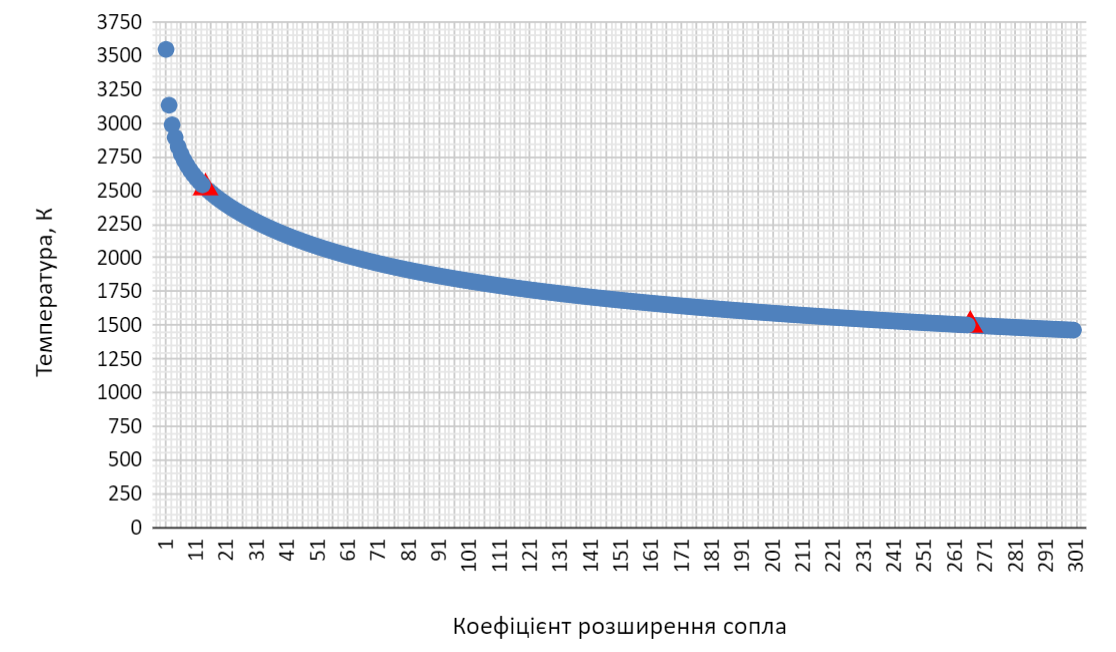
\includegraphics[width=0.7\textheight, angle=0,origin=c]{chapter_3/SV3_T(epsilon).png}
	\caption{Профіль температури у соплі двигуна SV3; червоним показані перерізи розташування МПД-каналу}
	\label{fig:SV3_T(epsilon)}
\end{figure}

\begin{figure}
	\centering
	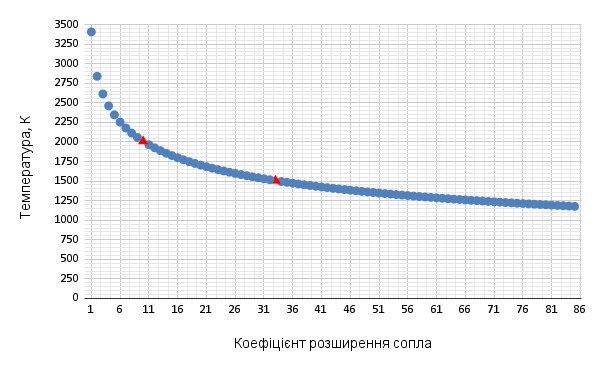
\includegraphics[width=0.7\textheight, angle=0,origin=c]{chapter_3/RD-0120_T(epsilon).png}
	\caption{Профіль температури у соплі РД-0120; червоним показані перерізи розташування МПД-каналу}
	\label{fig:RD-0120_T(epsilon)}
\end{figure}

%Залежність геометрії каналу від температури у соплі як основний чинник зв'язку РРД і МПДП
%Розрахунок в Астрі для визначення взаємного розташування РРД і МГДП (переріз сопла)

Однією з ключових конструктивних проблем рушійної установки, що розглядається у цій роботі, є визначення місця установки МПД-каналу у поздовжньому перерізі РРД. Частинки калію є іонізованими за певних значень температури їх потоку (діапазон $3000 - 1500$~K за даними~\cite{Panchenko}), а отже електромагнітне поле має бути прикладене у перерізі РРД з температурою у цьому діапазоні. Окрім цього з результатів CFD-моделювання у попередньому дослідженні~\cite{Previous} було якісно помічено, що частинки можуть вступати у термодинамічну рівновагу з потоком газу, а отже у критичному перерізі сопла вони набуватимуть швидкості, не більшою за швидкість потоку продуктів згоряння, тому їх електромагнітне прискорення до критики неможливе. Тому у складі плазморідинного двигуна МПД-прискорювач і його канал має бути розташований у закритичному перерізі сопла, на довжину, що відповідає температурі перерізу потоку робочого тіла $1500-3000$~K.

Для визначення меж розташування каналу також був використаний розрахунок з програмного пакету \texttt{Астра.4/рс}: для двигунів за визначеними раніше термодинамічними параметрами (11Д123, SV3 і РД-0120) були отримані профілі температури у ядрі потоку по осі сопла РРД, зображені на рис.~\ref{fig:11D123_T(epsilon}, ~\ref{fig:SV3_T(epsilon)} і ~\ref{fig:RD-0120_T(epsilon)} відповідно. Червоним відмічені перерізи установки каналу у межах, що відповідають ступеню іонізації частинок присадки, близькому до одиниці, за оптимального тиску для роботи МПД-каналу (за даними~\cite{Panchenko}, для лужних металів і температур РРД 10 бар та нижче відповідно).

Після визначення місця розташування МПД-каналу для розглянутих у розділі~\ref{sec:model_conditions} двигунів з урахуванням параметрів МГД-установок, зазначених у~\cite{MHDG}, були розраховані робочі об'єми каналу; ці величини прямо впливають на тягу прискорювача, оскільки ними обмежується переріз, у якому на присадку діє поле електродів та котушок установки.


\section{Оцінка характеристик МПД-прискорювача}

\subsection{Живлення установки\label{sec:power_supply}}

% опис роботи комплексу ТНА+МГДП
Для генерації електромагнітного поля і надання швидкостей робочого тіла у декілька км/с прискорювач потребує підведення потужності порядку мегават. В установці, що розглядається, ця потужність була б доступна на валу системи подачі палива РРД за умови її надлишкової генерації турбіною газогенератора. Проте більшість циклів роботи РРД не дозволяють здійснити відбір потужності (ця проблема розглянута у розділі~\ref{sec:First}).

Для оцінки потужностей, необхідних для отримання високої швидкості витікання МПД-прискорювача, можемо використати термодинамічні параметри двигунів, що розглядались вище (табл.~\ref{tab_LPRE}), а також за допомогою пакету \texttt{Астра.4/рс} розрахувати характеристики газогенератора, необхідного для генерації потужності окремої, паралельної турбіни для живлення МПД-прискорювача. Після генерування потужності на валу турбіни вона може бути перетворена у корисну із застоcуванням синхронного електрогенератора на постійних магнітах -- сучасні установки такого типу дозволяють досягти масової ефективності понад 25 кВт/кг~\cite{PMSG}. Результати оцінки на основі розрахованих ТД-параметрів газогенераторів на відновному газі (потужність турбіни та витрата палива для її роботи) наведені у табл.~\ref{tab_MHD}.

\begin{table}[t!]\centering\small
	\caption{Параметри МПД-установок для РРД різних потужностей (згідно характеристик аналогічних пристроїв~\cite{MHDG})}
	\begin{tblr}{|X[5cm]|Q[3cm]|Q[3cm]|}
		\hline
		& РД-0120 (паралельна турбіна) &  Flight Control SV3 (з водневою турбіною живлення)	\\
		\hline
		Паливо                     & LH2+LOX & Jet A-1+LOX / LH2+LOX \\
		\hline
		Корисна потужність турбіни живлення, МВт                   & 16,817   L &  2,9    \\
		\hline
		Витрата на турбіну живлення (без урахування допалювання), кг/с           & 12,876   & 2,221   \\
		\hline
		Тяга, тс                   & 2,463	 & 1,297  \\
		\hline
		Витрата присадки (частка 2\%), кг/с     & 1,2045    & 0,2079  \\
		\hline
		Швидкість витікання, м/с   & 20054,768  &  61180,736 \\
		\hline
	\end{tblr}
	\label{tab_MHD}
\end{table}



Потужність турбіни живлення залежить від параметрів газу, що поступає на неї з газогенератора (ГГ); чим більшу внутрішню енергію має паливо, тим більша питома потужність установки. Для порівняння були взяті газогенератори двигунів РД-0120 (водневий високого тиску на відновлювальному газі) та 11Д123 (РД-120, паливна пара керосин-кисень, на окиснювальному газі); дані по параметрах газогенераторів взяті з джерел~\cite{Fatuyev, RD-0120}. Оцінка проводилась з огляду на коефіцієнт корисної дії активних турбін РРД розглянутих класів та синхронних генераторів на постійних магнітах. Для водневого газогенератора РД-0120 значення газової сталої продуктів згоряння майже на порядок перевищує цей показник у керосинового ГГ РД-120; потужність на валу водневої турбіни дозволяє отримати прийнятні значення потужності за допустимої витрати палива, керосинова ж турбіна має надто велике споживання. Для 11Д123 з оцінки випливає потреба у витраті на турбіну живлення МПД-установки близько 70\% сумарної витрати самого РРД, що виключає будь-яку доцільність використання МПД-каналу у цьому двигуні.

Витрата палива для генерації корисної потужності у випадку двигуна РД-0120 з урахуванням подальшого допалювання у КЗ становить 12~\% від витрати основної турбіни ТНА РРД. У випадку SV3 воднева турбіна для отримання належної для роботи МПД-каналу густини потужності потребуватиме більше палива, ніж сам РРД (125\% основної витрати двигуна з урахуванням допалювання у КЗ), отже у конструкції цього двигуна застосування МПД-установки також стає недоцільним.

%Отримані результати дають змогу оцінити доцільність використання МПД-прискорювача з огляду на порядок приросту тяги та питомого імпульсу.

%З отриманих значень  температури у камері можемо розрахувати питомий імпульс (теоретичний, без урахування основних втрат, оскільки такі вже були враховані під час моделювання; найбільш значущими є радіаційний теплообмін стінок камери і вплив турбулентності на горіння). Також зі значень швидкості потоку і спаду тиску на зрізі сопла можемо знайти тягу двигуна.


\subsection{Оцінка тяги та швидкості витікання}


%струм на електродах з густини потужності
%потужність прискорювача з геометрії МПД-каналу
%геометрія (довжина каналу) і потужність диктують тягу і швидкість витікання присадки

%Розрахунок потужності МГД-прискорювача граничних параметрів;
%охолодження установки
За умови надання необхідної електричної потужності з генератора на валу турбонасосного агрегата (ТНА) РРД МПД-прискорювач отримує певну частку енергії з циклу рідинного двигуна, перетворюючи її у кінетичну енергію потоку заряджених частинок присадки калію. Тяга, створена таким потоком, незначна внаслідок малої частки присадки у потоці газу, проте вона може мати значно більшу швидкість, що дозволяє отримати більший питомий імпульс установки за умови компенсації втрат на іонізацію калію у потоці робочого тіла РРД.

Маючи розраховану потужність турбіни живлення та корисну потужність, що подається на МПД-канал з генератора (розглянуті у розділі~\ref{sec:power_supply}), можливо оцінити параметри струму на електродах прискорювача і відповідно густину струму в МПД-каналі. Потужність самого прискорювача також диктується геометрією МПД-каналу, оскільки поле створюється у визначеному об'ємі; це визначає силу, яка діє на потік заряджених частинок, що проходять у перерізі каналу і відповідно створюють реактивну тягу, витікаючи з визначеною швидкістю. У рамках оціночного розрахунку рух частинок присадки вважається прямолінійним.

%Розрахунок оптимального співвідношення “тяга-швидкість витікання” для діапазону процентів присадки

\begin{figure}
	\centering
	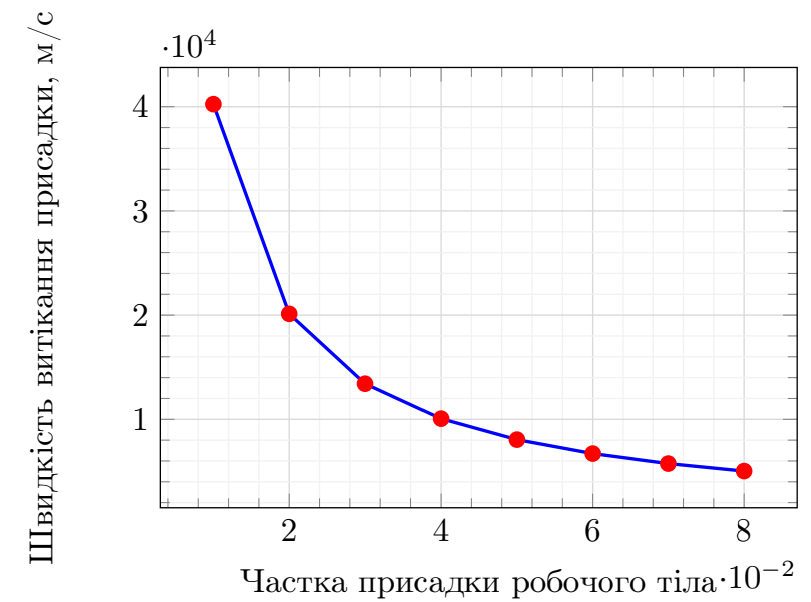
\includegraphics[width=0.5\textheight, angle=0,origin=c]{chapter_3/plot_Isp_WF.png}
	\caption{Графік залежності швидкості витікання робочого тіла МПД-прискорювача від витрати присадки у робочому тілі двигуна (РД-0120, режим низької тяги, РРД дросельований)}
	\label{fig:plot_Isp_WF}
\end{figure}

Тяга МПД-прискорювача була оцінена з виразу для пондеромоторної сили, що діє на електропровідний потік присадки у поздовжньому перерізі на осі МПД-каналу (ідеальний випадок) і утворена взаємодією схрещених електричного та магнітного полів (див. розділ~\ref{sec:First}):

\begin{equation*}
P_{MPD} = j~B \sin{\alpha},
\end{equation*}

де $j$ --- густина струму у перерізі каналу (поздовжньому), $B$ --- індукція котушок, $\alpha$ --- кут між лініями електричного й магнітного полів на осі каналу (конструктивно зумовлено, що на осі МПД-каналу $\alpha = 90\deg$).

Теоретична густина струму на електродах МПД-прискорювача розраховується за формулою (супутніми явищами типу ефекту Холла та ін. нехтуємо):

\begin{equation*}
	j = \frac{I}{F_{el}},
\end{equation*}

де $I$ --- струм на розгінних електродах, $F_{el}$ --- площа поздовжнього перерізу каналу.

Тяга МПД-прискорювача пов'язана з витратою та швидкістю витікання (у випадку електричного ракетного двигуна вона ж є питомим імпульсом у м/с) наступним співвідношенням:

\begin{equation*}
	P_{MPD} = v_{e}~\dot{m}_{MPD},
\end{equation*}

де $v_{e}$ --- швидкість витікання РТ (чисельно дорівнює питомому імпульсу ЕРД), $\dot{m}_{MPD}$ --- масова витрата РТ прискорювача.

Параметри МПД-установки, оцінені згідно геометрії сопла РРД, у якому розташовується МПД-канал, та характеристик створених електричного і магнітного полів, наведені у табл.~\ref{tab_MHD}.

З отриманого перерізу МПД-каналу, використавши електричну потужність прискорювача, можна оцінити густину струму у каналі і відповідно тягу МПД-компонента установки. Для двигуна з-поміж розглянутих вище РРД з допустимою витратою палива для живлення (РД-0120) тяга встановленого у соплі прискорювача становить близько 2,5 тс за значення масової частки присадки 2\%. Тягу можливо підвищити, збільшивши процент присадки, проте це знизить кінетичну енергію потоку РРД і швидкість витікання потоку присадки, оскільки параметри прискорюючого поля диктуються доступною для роботи установки електричною потужністю. Залежність швидкості витікання робочого тіла МПД-прискорювача від частки присадки наведена на рис.~\ref{fig:plot_Isp_WF}.

Результати оцінки (характеристики плазморідинної силової установки на основі РД-0120) наведені у табл.~\ref{tab_PFRE}.

\begin{table}[t!]\centering\small
	\caption{Характеристики гібридної рушійної установки на основі вибраного РРД}
	\begin{tabular}{|l|c|}
		\hline
		& РД-0120 (паралельна турбіна) \\
		\hline
		Частка витрати на турбіну живлення, \% & 2,57 \\
		\hline
		Тяга РРД на другій ступені, тс         &  27,956 \\
		\hline
		Тяга МПД-прискорювача, тс              &  2,463 \\
		\hline
		Швидкість витікання присадки (частка 2\%), м/с   & 20054,768 \\
		\hline
		Питомий імпульс РРД, м/с   							& 4567,977  \\
		\hline
		Приріст питомого імпульсу (РРД + МПД-прискорювач), \%   &   6,67\% \\
		\hline
	\end{tabular}
	\label{tab_PFRE}
\end{table}



В установці пропонується використання надпровідних котушок для зменшення уже наявного (внаслідок близького розташування КЗ) значного теплового навантаження; це дозволить мінімізувати втрату корисної потужності в елементах МПД-прискорювача. Струм на електродах розрахований з потужності, поданої на прискорювач, індукція магнітного поля і напруга підібрані з урахуванням параметрів аналогічних установок~\cite{MHDG}. Ефективність установки можна покращити шляхом додавання контуру регенеративного охолодження котушок; це дозволить збільшити температуру пального на вході у камеру, підвищуючи характеристики РРД на величину порядку 1-2\%.

%Питомий імпульс двигуна розраховується за формулою (подана у~\cite[с. 86]{Walther}):
%\begin{equation*}
%g I_{sp} = v_{e, max} = \sqrt{(n + 2) \frac{R T_{0}} {M_{p}}} ,
%\end{equation*}
%де $g$ --- прискорення вільного падіння, $I_{sp}$ --- питомий імпульс, $v_{e, max}$ --- максимальна ефективна швидкість витікання, $n$ --- показник ступеня свободи молекул газу в суміші продуктів згоряння (у даному випадку для суміші РРД $n = 7,41$), $R$ --- універсальна газова стала, $T_{0}$ --- температура у КЗ, $M_{p}$ --- молярна маса продуктів згоряння (для суміші РТ даного РРД 17,473 г/моль, з урахуванням присадки збільшується до 17,864 г/моль).

%Тяга двигуна розраховується за формулою~\cite[с. 88]{Walther}:
%\begin{equation*}
%F_{t} = \dot{m}_p v_{e} + (p_{e} - p_{\infty}) A_{e},
%\end{equation*}
%де $F_{t}$ ---  тяга, $\dot{m}_p$ --- масова витрата палива, $v_{e}$ --- ефективна швидкість витікання РТ, $p_{e}$ --- тиск на зрізі сопла, $p_{\infty}$ --- тиск навколишнього середовища, $A_{e}$ --- площа соплового зрізу.

%Знак між членами характеризує лише осьову компоненту швидкості (у даному випадку другий доданок з різницею тисків від'ємний через недорозширення сопла).

\section{Перспективи використання РРД з МГД-прискорювачем}

\begin{figure}
	\centering
	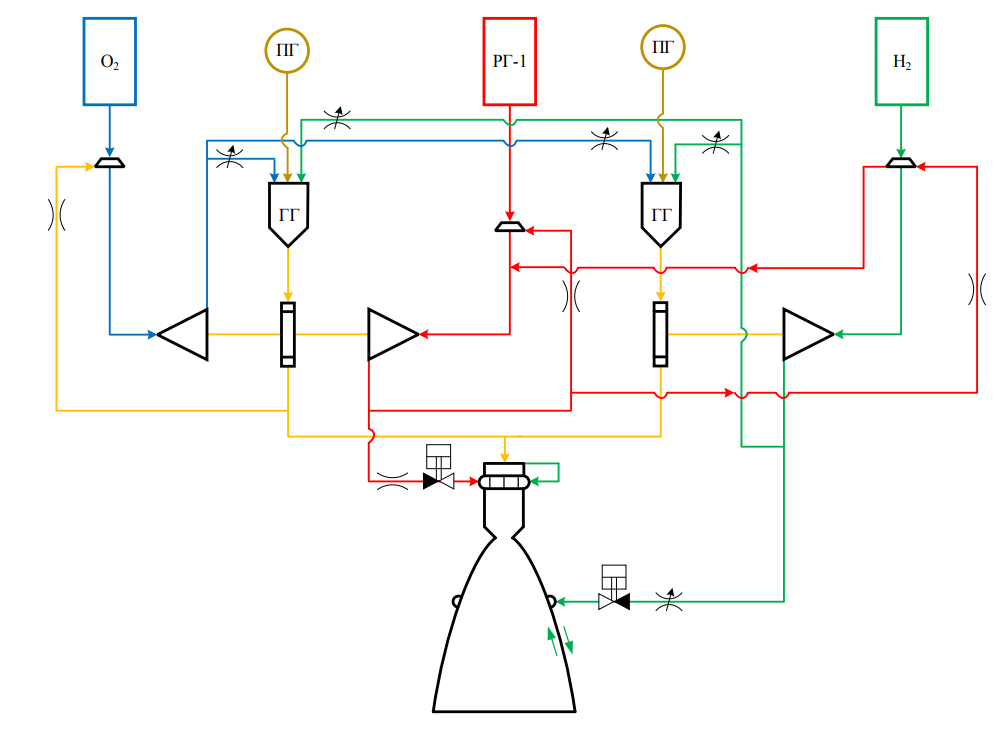
\includegraphics[width=0.6\textheight, angle=0,origin=c]{chapter_3/3comp_engine.png}
	\caption{Принципова схема дворежимного трикомпонентного ракетного двигуна РД-701; на другому режимі використовується воднева турбіна}
	\label{fig:3comp_engine}
\end{figure}

\begin{figure}[h!]
	\centering
	\subfloat[Типовий РРД верхніх ступеней (широкий пунктир)]{%
		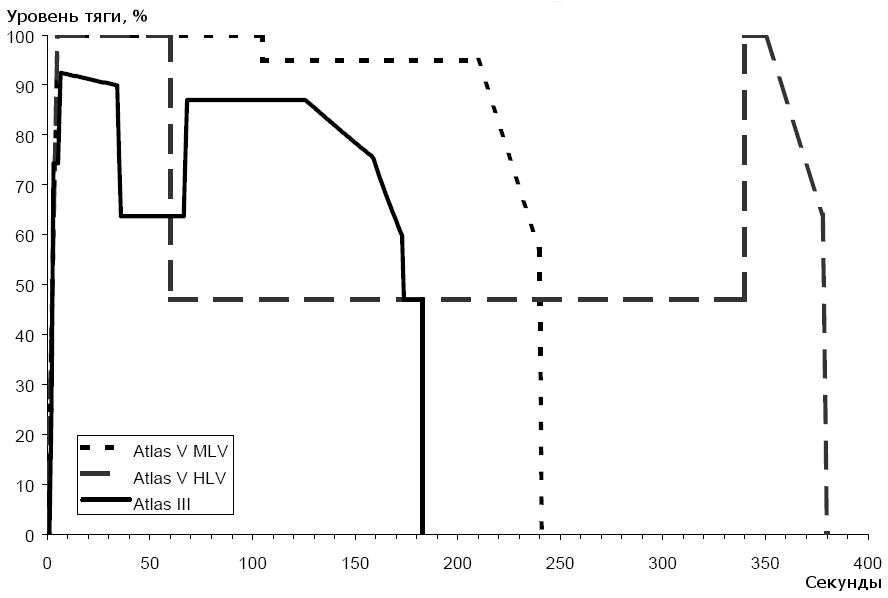
\includegraphics[width=0.6\columnwidth]{chapter_3/RD-180_cyclogram.jpg}
		\label{RD-180_cyclogram}
	}%
	\\ % <- для того, щоб рисунки розташувались в колонку
	\subfloat[Плазморідинний РД]{
		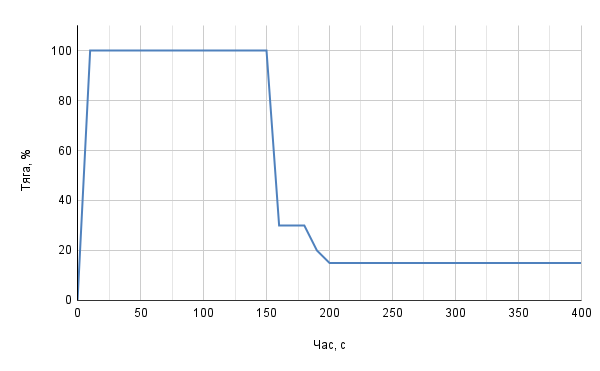
\includegraphics[width=0.6\columnwidth]{chapter_3/thrust_profile_PFRE.png}
		\label{thrust_profile_PFRE}
	}%
	\\
	\caption{Профілі тяги типового РРД верхньої ступені ракети-носія (а) і плазморідинного двигуна у двоступеневій схемі (перша ступінь -- робота РРД, друга ступінь -- глибоко дросельований РРД паралельно з МПД-прискорювачем)}
\end{figure}

%моделювання магнітної системи
%моделювання ерозії критики
%максимізація проценту присадки

Для оцінки параметрів МПД-прискорювача у складі плазморідинного двигуна використовувались зазначені вище три зразки РРД: високоенергетичний великої потужності (РД-0120), висотний керосиновий великої потужності (РД-120) і двигун верхньої ступені з порівняно меншою тягою (Flight Control SV3).

Були розраховані спад тяги і питомого імпульсу РРД внаслідок додавання присадки, корисна потужність на МПД-прискорювач і відповідно отримана тяга та питомий імпульс гібридної установки.

Варто зазначити, що витрати палива для отримання електричної потужності не у всіх трьох розглянутих випадках є оптимальними (у випадку SV3 витрата сягає значень номінальної для РРД на режимі, що виключає можливість ефективного використання ТНА; для 11Д123 МПД-прискорювач недоцільний через неоптимальну геометрію для МПД-каналу у соплі та необхідність додавання масивної водневої паливної системи). Двигун верхньої ступені на парі LH2 + LOX може бути більш придатним для використання у складі розглянутої електрохімічної рушійної установки.

Для компенсації втрат ентальпії потоку продуктів згоряння РРД в установці наявна можливість догріву пального окремим контуром регенеративного охолодження для компенсації спаду імпульсу (у випадку SV3 нагрів на $200$~К повністю компенсує втрату тяги камери).

Існує альтернативний цикл роботи РРД --- трикомпонентна схема, за якої використовуються два ТНА для трьох різних компонентів палива (це дозволяє підвищити масову ефективність і питомий імпульс на різних ділянках польоту, використовуючи два різних види пального з одним окиснювачем) (рис.~\ref{fig:3comp_engine}). Другий ТНА цього двигуна можна використати під час його простою для отримання потужності для МПД-прискорювача, таким чином РРД стає однорежимним (рис.~\ref{RD-180_cyclogram}), або ж має два режими (рис.~\ref{thrust_profile_PFRE}):

\begin{itemize}
	\item великої потужності (працюють обидва ТНА, МПД-прискорювач вимкнено);
	\item високоефективний режим малої тяги (працює один ТНА на більш високоенергетичному компоненті + МПД-прискорювач).
\end{itemize}

Існує протестований зразок дворежимного трикомпонентного двигуна на компонентах РГ-1 + LH2 + LOX --- РД-0750~\cite{RD-0120}. За попередньою оцінкою, використовуючи другий водневий газогенератор такого РРД, можна отримати потужність для МПД-прискорювача порядку 15\% від потужності ТНА спряженого РРД. Для випадку газогенератора РД-0750 витрата, необхідна для отримання потужності, що подаватиметься на МПД-прискорювач, становить близько 13\% витрати двигуна на номінальному режимі.

Отримані результати дають змогу оцінити доцільність використання МПД-прискорювача з огляду на порядок приросту тяги та питомого імпульсу РРД у розглянутій гібридній рушійній установці.

Наведена оцінка потребує подальшого уточнення за допомогою CFD-моделювання МПД-каналу у поєднанні з газодинамічним трактом РРД і взаємодії прискорених іонізованих частинок присадки з надзвуковим потоком продуктів згоряння РРД за наявності схрещених електричного та магнітного полів. Також потребується врахування складної конструкції магнітної системи котушок складної форми (вигнутої по формі сопла РРД). Важливим є питання ерозії стінок камери і сопла за присутності калію для оцінки ресурсу роботи рушійної установки визначених параметрів. Уточнення вищеозначених аспектів моделі дозволить оптимізувати співвідношення робочих тіл РРД і МПД-прискорювача, збалансувавши тягу та питомий імпульс складових розглянутого концепту рушійної установки літального апарата.


\section{Висновки розділу 3}

%Проведене дослідження зміни тяги та питомого імпульсу РРД при введенні у камеру присадки калію шляхом моделювання двофазного потоку з дискретною фазою та виведення основних його характеристик для отримання відповідних параметрів двигуна.

Наведені результати енергетичного розрахунку та термодинамічних параметрів трьох різних РРД, без введення присадки та за її наявності. Розрахований спад тяги двигунів, пов'язаний з введенням робочого тіла МПД-установки у паливну суміш.

На основі результатів ТД-розрахунку були виведені профілі температур по осі сопла, що дозволило розрахувати доступний об'єм МПД-каналу для прискорювача.

Була розрахована потужність турбіни живлення МПД-прискорювача на основі характеристик водневого газогенератора двигуна РД-0120, була оцінена доступна електрична потужність для плазморідинного двигуна.

Було визначено тягу та питомий імпульс МПД-прискорювача для двигуна РД-0120; окреслено недоцільність компонування МПД-компонентом двох інших РРД внаслідок надмірної витрати палива для живлення.

Результати моделювання та подальшої кількісної оцінки свідчать про те, що приріст ефективності плазморідинного двигуна залежить у першу чергу від доступної для МПД-прискорювача потужності, для масових часток присадки порядку декількох процентів витрати РРД спад характеристик рідинного двигуна є незначним, проте для істотного підвищення параметрів МПД-компонента необхідна значно більша потужність, ніж може дати паралельно встановлена воднева газова турбіна.

При розв'язанні проблеми компактного енергоносія для ЕРД плазморідинний двигун може бути ефективним дворежимним РД верхньої ступені ракети-носія внаслідок високої швидкості витікання робочого тіла установки.